\documentclass{article}

% Language setting
% Replace `english' with e.g. `spanish' to change the document language
\usepackage[english]{babel}

% Set page size and margins
% Replace `letterpaper' with `a4paper' for UK/EU standard size
\usepackage[letterpaper,top=2cm,bottom=2cm,left=3cm,right=3cm,marginparwidth=1.75cm]{geometry}

% Useful packages
\usepackage{amsmath}
\usepackage{chronology}
\usepackage{tikz}
\usepackage{pgfplots} 
\usetikzlibrary{mindmap,trees, patterns}
\usepackage{graphicx}
\usepackage{smartdiagram}
\usepackage{float}
\usepackage[colorlinks=true, allcolors=blue]{hyperref}
\usepackage{multirow,tabularx}
\usepackage{amsthm}
\usepackage{hyperref}
\usepackage{nameref}
\pgfplotsset{compat=1.18}
\title{RockX ETH2.0 Liquid Staking Explained}
\author{RockX Team}

\begin{document}
\maketitle

\begin{abstract}
Staking, a cryptoeconomic primitive that allows participants to earn yield in exchange for locking tokens, has taken center stage over the past two years. Under a Proof of Stake consensus mechanism, instead of using computational power, validators lock (“stake”) a certain amount of the network’s native cryptoasset as collateral, thus becoming eligible to create new blocks. In return, they earn inflationary rewards and transaction fees.
\end{abstract}

\section{Introduction}

\subsection{What is Proof of Stake?}

Proof of Stake is the consensus protocol utilised in Ethereum 2.0 (ETH2). The consensus protocol helps everyone to know what transactions have been processed and in what order, which is known as validation.\

ETH2 currently has a Proof of Stake (PoS) chain called the Beacon Chain, which is faster, more energy efficient and more decentralised than the current consensus protocol Ethereum is utilising (Proof of Work). Users deposit ETH and provide an Ethereum node to perform the required validation. As a reward for providing the node, the Beacon Chain gives node operators additional ETH on top of their deposits. These rewards are minted in return for helping secure the network.

\subsection{What is liquid staking?}

It is clear that PoS chains will be an integral part of the future of crypto, and become the foundation layer of which DeFi and metaverses will be built on.

However, PoS comes with some drawbacks for those wanting to participate directly as validators:

It requires technical know-how to set up and operate a node and the required $32\cdot ETH$ deposit are significant barriers for regular token holders to participate in PoS validation. Staked tokens are locked up and become illiquid assets. In order to solve these issues, liquid staking protocols were born. Liquid staking abstracts the depositing of tokens from running a validator node.

In exchange for their tokens, depositors receive a representative (uniETH) token from the protocol which is a claim on the tokens they have staked.

\subsection{What is uniETH?}

uniETH represents the staked ETH plus all future staking rewards. uniETH does not grow in quantity over time but instead, grows in value, i.e. $1\cdot uniETH$ becomes worth increasingly more than $1\cdot ETH$. If you deposit $1\cdot ETH$ initially, then your $1\cdot uniETH = 1\cdot ETH$, however after receiving some rewards and the total claim you have is $1\cdot ETH + 0.2\cdot ETH$ rewards, then your $1\cdot uniETH = 1.2\cdot ETH$.

\subsection{How are staking rewards distributed?}
As all the ETH deposited through this protocol is pooled together to provide the $32\cdot ETH$ for each node, the node will receive the rewards and automatically distribute it across all staking participants based on how much ETH they staked of the 32 ETH total. I.e. if you staked 3.2 ETH you will receive 10\% of each reward.
Each time rewards are distributed (every block), they will be added to the initial stake amount, eventually compounding future earnings as more nodes are added, while immediately increasing the value of the uniETH tokens representing each stake.


\subsection{What should I stake with RockX instead of staking directly to ETH2?}

RockX removes several drawbacks that exist with Proof of Stake on ETH2.
The Beacon Chain requires a minimum deposit of at least $32\cdot ETH$. RockX will allow anyone to earn rewards on any amount of ETH deposited with us.
When depositing ETH on the Beacon Chain, users are required to have technical knowledge of interacting with smart contracts. RockX handles all interaction with the Beacon Chain for our users. The Beacon Chain will also require users who make deposits to be technically proficient at running Ethereum nodes, keeping their own node online and secure 24/7. RockX provides this service for our users.
					
As ETH2 is being rolled out in several phases. We are currently in phase 1, the merge, and depositing now means your deposit is locked until phase 2 arrives, which could very well still be a long time away. With RockX you instantly get uniETH when depositing and do not need to be locked with us. uniETH can be held, traded, or sold at any time, providing our users with instant liquidity on their staked ETH.

\subsection{What is the staking period for uniETH?}
The staking period to redeem the underlying ETH with uniETH will only be confirmed once ETH2 goes into phase 2. However, you will instantly receive uniETH when you deposit ETH and you will still gain staking rewards over time as your uniETH will increase in value as your rewards are added to your initial stake. uniETH can also be sold and traded on various DEXs and CEXs if there is liquidity available for the trade.

\subsection{What is the minimum deposit?}
RockX gives everyone the opportunity to earn rewards on any amount of ETH, as we do not have a min- imum. We do recommend a deposit of at least 0.01ETH to make your transaction worthwhile. When you stake ETH, you will receive uniETH, which gains rewards over time based on the performance of our nodes on the Beacon Chain.

\subsection{What is the maximum deposit?}   
There is no limit on the amount of ETH you can stake with RockX on ETH2. The more ETH you stake, the more rewards you will receive.

\section{RockX uniETH staking algorithm}

\subsection{Terminology}
\begin{description}
   \item[ETH] $1\cdot ETH \equiv 10^{18}$
   \item[TotalSupply] current total supply of uniETH, the total supply of uniETH is proportional to total ETH staked.
   \item[TotalStaked] total 
 staked to validators.
   \item[TotalDebts] total unpaid debts, generated from \textbf{redeemFromValidators()}, awaiting to be paid by turning off validators and debt clearance procedure.
   \item[TotalPending] pending ETH to be staked.
   \item[RewardDebts] the remaining ETH from debt clearance procedure.
   \item[UserRevenue] overall net revenue which belongs to all uniETH holders.
   \item[ReportedValidators] latest reported active validators.
   \item[ReportedValidatorBalance] latest reported overall balance of active validators.
   \item[RecentEthersMoved] the amount this contract receives recently from validators.
   \item[CurrentReserve] overall assets under management, given as:
   \[CurrentReserve = TotalPending + TotalStaked + UserRevenue - TotalDebts - RewardDebts\]
   \item[Exchange Ratio] Defined as symbol $\rho$ of uniETH to ETH, given as: 
   \begin{equation}
    \rho = \begin{cases}
        \frac{TotalSupply}{CurrentReserve} & \text{ $ CurrentReserve \in (0, +\infty) $}\\
        1 & \text{ $ CurrentReserve = 0 $}
    \end{cases}
    \end{equation}
    normally: $\rho \leq 1.0$
   \item[managerFeeShare] share of the manager fee, represented as 1 in 1000, managerFeeShare $\in[0,1000]$ 
\end{description}

\newtheorem{theorem}{Theorem}[section]
\newtheorem{corollary}{Corollary}[theorem]
\newtheorem{lemma}[theorem]{Lemma}

\begin{figure}
\begin{center}
    \smartdiagram[circular diagram:clockwise]{register validators, mint, delegation, push rewards, redeem, claim, validators exit}
\end{center}
\caption{Lifecycle of RockX Staking Contract.}
\end{figure}

In the sections below, we'll explain the details of liquid staking from a user's perspective.

\subsection{Stake ETH to mint uniETH}
A user calls function \textbf{mint()} with a specific amount of \textbf{ethersToStake} ETH to mint \textbf{uniETH}, in each function call, we have:

\begin{theorem}
\label{Mint}
\[minted_{uniETH} := \rho \cdot ethersToStake \]
\[TotalSupply = TotalSupply^{\prime} + minted_{uniETH} \]
\[TotalPending = TotalPending^{\prime} + ethersToStake\]
\end{theorem}

Users receives \underline{$minted_{uniETH}$} token of uniETH  if \textbf{mint()} succeeds. \textbf{uniETH} is a standard \textbf{ERC-20} compliant contract issued only by RockX staking contract. Besides redeeming for the staked ETH through our smart contract, uniETH can also be traded on \textbf{DEX}s as long as there is sufficient liquidity on DEXs.

The general rule for \textbf{minting} and \textbf{redeeming} is: \underline{keep the exchange ratio - $\rho$ invariant}, if $\rho$ changes during \textbf{minting} and \textbf{redeeming} process, users can arbitrage.

\begin{proof}
To prove $\rho$ invariant and irrelevant of ETH to stake, for $CurrentReserve \in (0, +\infty)$:

\[\rho = \frac{TotalSupply}{CurrentReserve} = \frac{TotalSupply^{\prime} + \rho^{\prime} \cdot ethersToStake}{CurrentReserve^{\prime} + ethersToStake}\]

as by definition:

\[\rho^{\prime} = \frac{TotalSupply^{\prime}}{CurrentReserve^{\prime}}\]

we have:

\[\rho=\frac{CurrentReserve^{\prime} \cdot \rho^{\prime}  + \rho^{\prime} \cdot ethersToStake}{CurrentReserve^{\prime} + ethersToStake} = \frac{\rho^{\prime} \cdot (CurrentReserve^{\prime} + ethersToStake)}{CurrentReserve^{\prime} + ethersToStake} \]

finally:

\[\rho = \rho^{\prime}\]

\end{proof}

\subsection{Initiating depositing into ETH2 offical contract}
\label{depositing}
At any time \textbf{TotalPending} has more than $32\cdot ETH$, the contract manager can call \textbf{stake()} function to stake the ETH into Ethereum 2.0 staking contract. As a result, $ETH$ in \textbf{TotalPending} moves to \textbf{TotalStaked} and keeps \textbf{TotalPending} less than $32\cdot ETH$, we will calculate the changes as follows:

\begin{lemma}
\[ethersToDeposit := \lfloor\frac{TotalPending^{\prime}}{32ETH}\rfloor \cdot 32ETH\]
\end{lemma}

The ETH to deposit to ETH2 official contract is bounded to $N\cdot 32ETH$ as above, we define the depositing process as:

\begin{theorem}
\label{depositing_vars}
\[TotalPending = TotalPending^{\prime} - ethersToDeposit \]
\[TotalStaked = TotalStaked^{\prime} + ethersToDeposit \]
\end{theorem}

In depositing process \ref{depositing}, $\rho$ is kept invariant as \textbf{CurrentReserve} does not change, as:
\begin{multline}
CurrentReserve := \dots + (TotalPending^{\prime} - ethersToDeposit) + (TotalStaked^{\prime} + ethersToDeposit) \\
= \dots + TotalPending^{\prime} + TotalStaked^{\prime} 
\end{multline}

\subsubsection{Timing}
The timing for calling stake() contract function mainly considers maximising capital efficiency, if we stake prematurely, the cost for running a single validator is way too expensive. On the flipside, if we are slow to stake, the deposited ETH does not generate rewards during the period prior to it begin staked in the official ETH2 staking contract. Hence, there is a need to build an off-chain program to provide a seamless and comprehensive solution for staking, allowing maximum capital efficiency on assets while earning cryptonative yields.

\subsection{Redeeming staked ETH from official RockX smart contract}
Users call contract function \textbf{redeemFromValidators()} with a specific amount of \textbf{ethersToRedeem} ETH expected to redeem, the amount uniETH to be burnt is exactly to $N\cdot 32ETH$ worth of uniETH, then we have:
\begin{theorem}
\label{Redeem}
\[burned_{uniETH} := \rho \cdot ethersToRedeem \]
\[TotalSupply = TotalSupply^{\prime} - burned_{uniETH} \]
\[TotalDebts = TotalDebts^{\prime} + ethersToRedeem\]
\end{theorem}
Redeeming(or Unstaking) works as by turning off validators, waiting for the validators to be offline and returning the staked ETH to the contract. It's a time-consuming asynchronous process. The benefit from redeeming directly from this contract is that there's no slippage which you may face in a CEX or DEX. However as this process takes time, you have to be patient. Once the ETH is returned, you'll be notified\footnote{available on web staking portal, \url{https://unieth.rockx.com/}} to claim it.

$\rho$ is also invariant and irrelevant of ETH to unstake.

Note: redeeming function will only be available after ETH2.0 merged.

\subsection{How ETH return to this contract from validators? }
\label{sectionAccounting}

At current, Ethereum 2.0 withdrawals implementation are not like normal transactions. Instead, they are system level transactions that update an account's balance without a transaction in or out. In our contract implementation, we use \textbf{accountedBalance} to track explicit ETH in and out from contract functions, and compare \textbf{accountedBalance} with \textbf{this.balance}, the difference is the ETH rewards\footnote{Here we suppose nobody transfers ETH to this contract intentional or unintentional, if this happens, the contract treat the ETH as rewards, shared by all \textbf{uniETH} holders} returned from validators. We utilise variable \textbf{RecentEthersMoved} to track this difference:

\[RecentEthersMoved = accountedBalance - this.balance\]

Ethers moves from contract to validators, or vice versa, here we define: \textbf{RecentEthersMoved} is the ETH moved from ${validators}\Longrightarrow{contract}$. The balancing syncing is done in \textbf{syncBalance()}

\subsection{Stopping validators for debt clearance}
Whenever a validator is stopped by a node operator, the ETH are supposed to return to this contract due to the setting of \textsc{withdrawal\_credentials} in depositing \footnote{\nameref{depositing}}, once the ETH returned, the oracle calls \textbf{validatorStopped()} function, along with the following parameters:
\begin{description}
\item[valueStopped] The ETH sent-back from validators to the liquid staking contract.
\item[validatorStopped] The count of stopped validators.
\end{description}
Suppose:

\[valueStopped \geq amountUnstaked \]
and meanwhile, ETH in validators has been transferred to contract and \textbf{RecentEthersMoved} has been updated as explained in section:\ref{sectionAccounting}:
\[RecentEthersMoved = RecentEthersMoved^{\prime} + valueStopped\]

If we do not have \textbf{slashing}, then we can deduce from the parameters that:
\begin{lemma}
\[amountUnstaked := 32\cdot ETH \cdot validatorStopped\]
\[incrRewardDebt := valueStopped - amountUnstaked\]
\end{lemma}

and, we use the 2 varaibles above to update the following variables:
\begin{theorem}
\label{validatorStopped}
\[RewardDebts = RewardDebt^{\prime} + incrRewardDebt\]
\begin{multline}
TotalPending = TotalPending^{\prime} + incrRewardDebt \\
+ Max\{0, amountUnstaked - TotalDebts\}
\end{multline}
\[TotalStaked = TotalStaked^{\prime} -  amountUnstaked \]
\end{theorem}

\subsection{Calculating rewards}
Rewards are aggregated on a daily basis, and will be reflected from the decrease of \textbf{exchange ratio}-$\rho$, meaning you receive more ETH back.

\begin{chronology}[5]{1}{15}{90ex}
\event{1}{pushBeacon($32\cdot ETH$)}
\event{3}{pushBeacon($32.1\cdot ETH$)}
\event{6}{pushBeacon($32.3\cdot ETH$)}
\event{12}{pushBeacon($32.6\cdot ETH$)}
\end{chronology}

An oracle service running offchain will push overall alive validators balance periodically, there're 2 things \textbf{pushBeacon()} do to update the reward:

\subsubsection{Adjusting reward base}
Firstly, pushBeacon will check if any new validators has gone alive, the reward base will be adjusted to align to the newly staked ETH plus previously reported validators balance ETH, the \textbf{reward base} is defined as the \underline{reference point} to compare to current balance, and it'll be updated in each consecutive pushBeacon() call with current \textbf{aliveBalance}.

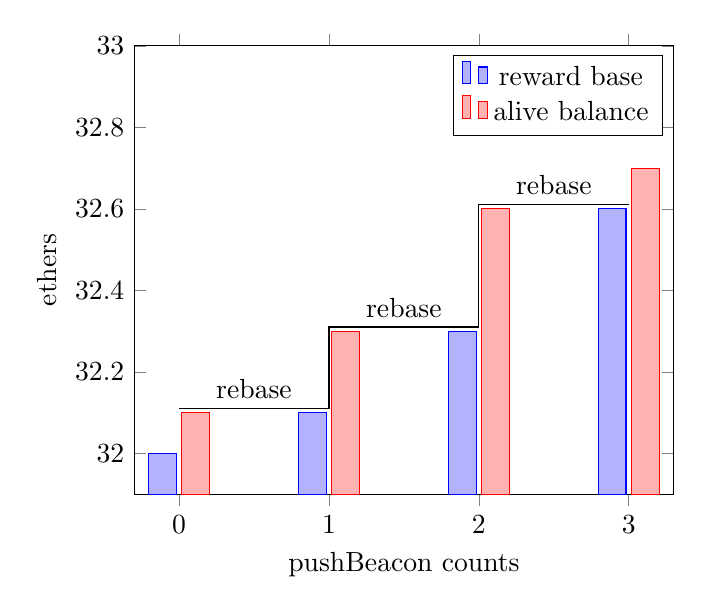
\begin{tikzpicture}
\begin{axis} [ybar,
    xtick = data,
    ymax = 33,
    xlabel = pushBeacon counts,
    ylabel = ethers,
]
 
\addplot coordinates {(0,32) (1,32.1) (2,32.3) (3,32.6)};
\addplot coordinates {(0,32.1) (1,32.3) (2,32.6) (3,32.7)};
\addplot[black,sharp plot,update limits=false] 
	coordinates {(0,32.11) (1,32.11) (1,32.31) (2,32.31) (2,32.61) (3,32.61)}
	node[above] at (axis cs:0.5,32.11) {rebase}
	node[above] at (axis cs:1.5,32.31) {rebase}
	node[above] at (axis cs:2.5,32.61) {rebase};
\legend {reward base, alive balance};
\end{axis}
\end{tikzpicture}

Given:
\begin{description}
\item[aliveValidator] The count of validators alive
\end{description}
we have:
\begin{theorem}
\label{pushBeacon}
\[RewardBase = ReportedValidatorBalance + Max\{0, aliveValidator - ReportedValidators\} \cdot  32\cdot ETH\]
\end{theorem}

\subsubsection{Reward distribution}
Normally ETH will either stay in contract or validators, hence the overall assets under management or TVL is as follows:
\[TVL := ethersInContract + ethersInValidators\]

During calculation of rewards changes, we only consider the balance change in alive validators, we can assume if the equation satisfies:
\[aliveBalance + RecentEthersMoved \geq RewardBase\]

then positive rewards have generated, we formalise the formula as below, given:

\begin{description}
\item[aliveBalance] The balance of current alive validators
\end{description}
we have:

\begin{theorem}
\label{calcReward}
\[r := Max\{0, aliveBalance + RecentEthersMoved - RewardBase\}\]
\[UserRevenue = UserRevenue^{\prime} + r \cdot \frac{(1000 - managerFeeShare)}{1000}\]
\[RecentEthersMoved = 0\]
\[ReportedValidators = aliveValidator\]
\[ReportedValidatorBalance = aliveBalance\]
\end{theorem}

As \textbf{RecentEthersMoved} will only be counted during reward distribution, the variable will be reset to 0 at the end of each \textbf{pushBeacon()} call. The exchange ratio - $\rho$ will go down by the change of \textbf{UserRevenue}, which allows the \textbf{uniETH} holder to get back more ETH when redeems.

\subsubsection{Manager's Fee Withdrawal}
Withdrawal before ETH2.0 merge is still not implemented yet, but here is the general process: 

As \textsc{withdrawal\_credentials} has set to the contract address, to withdraw the manager's fee from validators, the manager MUST submit a request of withdrawal from the contract. Once the ETH arrive, the manager can claim them. 

The key issue here is, does manager's withdrawal affects the calculation of rewards, as \textbf{aliveBalance} has reduced? The simple answer is - NO. The ETH moves from validators to the contract is accounted in \textbf{RecentEthersMoved}. It won't be an issue as long as RecentEthersMoved is accounted for, to make sure this happens, we'll call \textbf{syncBlanace()} to update RecentEthersMoved each time manager withdraws.

\subsection{Slashing}
Slashing is when a large portion of a validator's stake is removed from the network. This usually happens when a validator breaks the rules that are designed to prevent attacks on the network. Being slashed means that the validator will be forced to exit the beacon chain at some point in the future, receiving penalties until it does so.

Nobody expects slashing, but when it happens, the contract MUST handle it. Basically, users will face a sudden change of \textbf{exchange ratio - $\rho$}, in our implementation we made a tiny modification to handle this situation in \textbf{pushBeacon()} and \textbf{validatorSlashedStop()}

\subsubsection{Handling slashing in validatorSlashedStop()}
Given:
\begin{description}
\item[remainingEthers] The ETH left after slashing
\item[slashedAmount] The ETH slashed
\item[slashedValidators] The count of slashed validators.
\end{description}
we have:
\begin{theorem}
\[TotalPending = TotalPending^{\prime} + remainingEthers \]
\[TotalStaked = TotalStaked^{\prime} - 32\cdot ETH \cdot slashedValidators \]
\[RecentSlashed = RecentSlashed^{\prime} +  slashedAmount \]
\end{theorem}

$\rho$ will have a sudden changed due to the change of \textbf{TotalPending} and \textbf{TotalStaked} as:
\[\rho = \frac{TotalSupply}{CurrentReserve - 32\cdot ETH \cdot slashedValidators + remainingEthers } \]

\subsubsection{Modification of rewards calculation in pushBeacon()}
\begin{theorem}
\[r := Max\{0, aliveBalance + RecentEthersMoved + RecentSlashed - RewardBase\}\]
\[UserRevenue = UserRevenue^{\prime} + r \cdot \frac{(1000 - managerFeeShare)}{1000}\]
\[RecentEthersMoved = 0\]
\[RecentSlashed = 0\]
\[ReportedValidators = aliveValidator\]
\[ReportedValidatorBalance = aliveBalance\]
\end{theorem}
You may think it's a bit strange that we include \textbf{RecentSlashed} to rewards accumulating, just remember, $\rho$ has already been changed, and 
\textbf{aliveBalance} has been decreased by \textbf{slashedAmount}, at the moment of slashing, we can say:

\begin{multline}
r := Max\{0, (aliveBalance^{\prime} - slashedAmount) \\
+ RecentEthersMoved + slashedAmount - RewardBase\}
\end{multline}

\section{DAO Governance}
The DAO token currently not completed yet, the supposed scenario is to vote on the key parameters of staking contract, such as:

\begin{description}
   \item[Manager's Fee Setting] to vote to change manager's fee percentage
   \item[Qualified Validators Registration] to vote on validator keys proposed by other institutions, or to remove a validator.
	\item[Granting Roles] to vote to grant specific roles to account addresses, like: \textit{ORACLE\_ROLE, REGISTRY\_ROLE, MANAGER\_ROLE, PAUSER\_ROLE} 
	\item[Upgrading Contract] to vote to upgrade staking contract implementation, in case of critical issues or external
	\item[ETH2 Phase Change] to vote to switch to another phase of ETH2.0, which will enable redeeming such as.
\end{description}

The current staking contract has been implemented to be upgradable, using transparent proxy.

\section{Conclusion}
RockX ETH2.0 Liquid Staking gives everyone the opportunity to earn rewards on any amount of ETH,  and gains 
rewards over time based on the performance of our nodes on the Beacon Chain. Allowing retail users to
participate in ETH2.0 network maintainence works like Inclusive Financial system in real world. Besides stakers has 
the ability to hedge their uniETH tokens to avoid losing money.

The overall design of this liquid staking protocol treats funds security as a core goal when utilising the fund to earn rewards. The source code and architecture has already been open-sourced to the public.

\newpage
\appendix
\section{Balance Sheet Demo}
\begin{table}[!ht]
    \centering
    \begin{tabular}{p{0.2\linewidth} | p{0.3\linewidth}| p{0.1\linewidth}| p{0.2\linewidth}| p{0.2\linewidth}}
    \hline
        \textbf{Initial Stage}:  & ~ & ~ & ~ & ~ \\ \hline
        User A Stakes 32 ETH & \textbf{ASSETS} & ETH & \textbf{LIABILITY} & uniETH \\ \hline
        ~ & \textbf{User A Deposit} & 32 & User A uniETH & 32 \\ \hline
        ~ & Total Assets & 32 & Total Liability & 32 \\ \hline
        ~ & SwapRatio & ~ & ~ & 1 \\ \hline
        \multicolumn{5}{c}{} \\ \hline
        \textbf{Stage 1}:  & ~ & ~ & ~ & ~ \\ \hline
        Got 0.32 ETH Rewards & \textbf{ASSETS} & ETH & \textbf{LIABILITY} & uniETH \\ \hline
        ~ & User A Deposit & 32 & User A uniETH & 32 \\ \hline
        ~ & \textbf{Mining Rewards} & 0.32 & ~ & ~ \\ \hline
        ~ & Total Assets & 32.32 & Total Liability & 32 \\ \hline
        ~ & SwapRatio & ~ & ~ & 1.01 \\ \hline
        \multicolumn{5}{c}{} \\ \hline
        \textbf{Stage 2}:  & ~ & ~ & ~ & ~ \\ \hline
        User B Stakes 64 ETH & \textbf{ASSETS} & ETH & \textbf{LIABILITY} & uniETH \\ \hline
        ~ & User A Deposit & 32 & User A uniETH & 32 \\ \hline
        ~ & \textbf{User B Deposit} & 64 & User B uniETH & 63.36633663 \\ \hline
        ~ & Mining Rewards & 0.32 & ~ & ~ \\ \hline
        ~ & Total Assets & 96.32 & Total Liability & 95.36633663 \\ \hline
        ~ & SwapRatio & ~ & ~ & 1.01 \\ \hline
        \multicolumn{5}{c}{} \\ \hline
        \textbf{Stage 3}: & ~ & ~ & ~ & ~ \\ \hline
        User B transfer 32 uniETH to User C & \textbf{ASSETS} & ETH & \textbf{LIABILITY} & uniETH \\ \hline
        ~ & ~ & ~ & User A uniETH & 32 \\ \hline
        ~ & ~ & ~ & User B uniETH & 31.36633663 \\ \hline
        ~ & ~ & ~ & \textbf{User C uniETH} & 32 \\ \hline
        ~ & Total Assets & 96.32 & Total Liability & 95.36633663 \\ \hline
        ~ & SwapRatio & ~ & ~ & 1.01 \\ \hline
        \multicolumn{5}{c}{} \\ \hline
        \textbf{Stage 4}: & ~ & ~ & ~ & ~ \\ \hline
          User A unstakes equivalent 32 ETH value of uniETH & \textbf{ASSETS} & ETH & \textbf{LIABILITY} & uniETH \\ \hline
        ~ & Before Redeeming & 96.32 & User A uniETH & 32 \\ \hline
        ~ & ~ & ~ & User B uniETH & 31.36633663 \\ \hline
        ~ & ~ & ~ & User C uniETH & 32 \\ \hline
        ~ & \textbf{User A Redeems} & -32 & User A Burned & -31.68316832 \\ \hline
        ~ & Total Assets & 64.32 & Total Liability & 63.68316831 \\ \hline
        ~ & SwapRatio & ~ & ~ & 1.01 \\ \hline
    \end{tabular}
\end{table}

\section{Architecture Overview}
\begin{figure}[H]
\centering
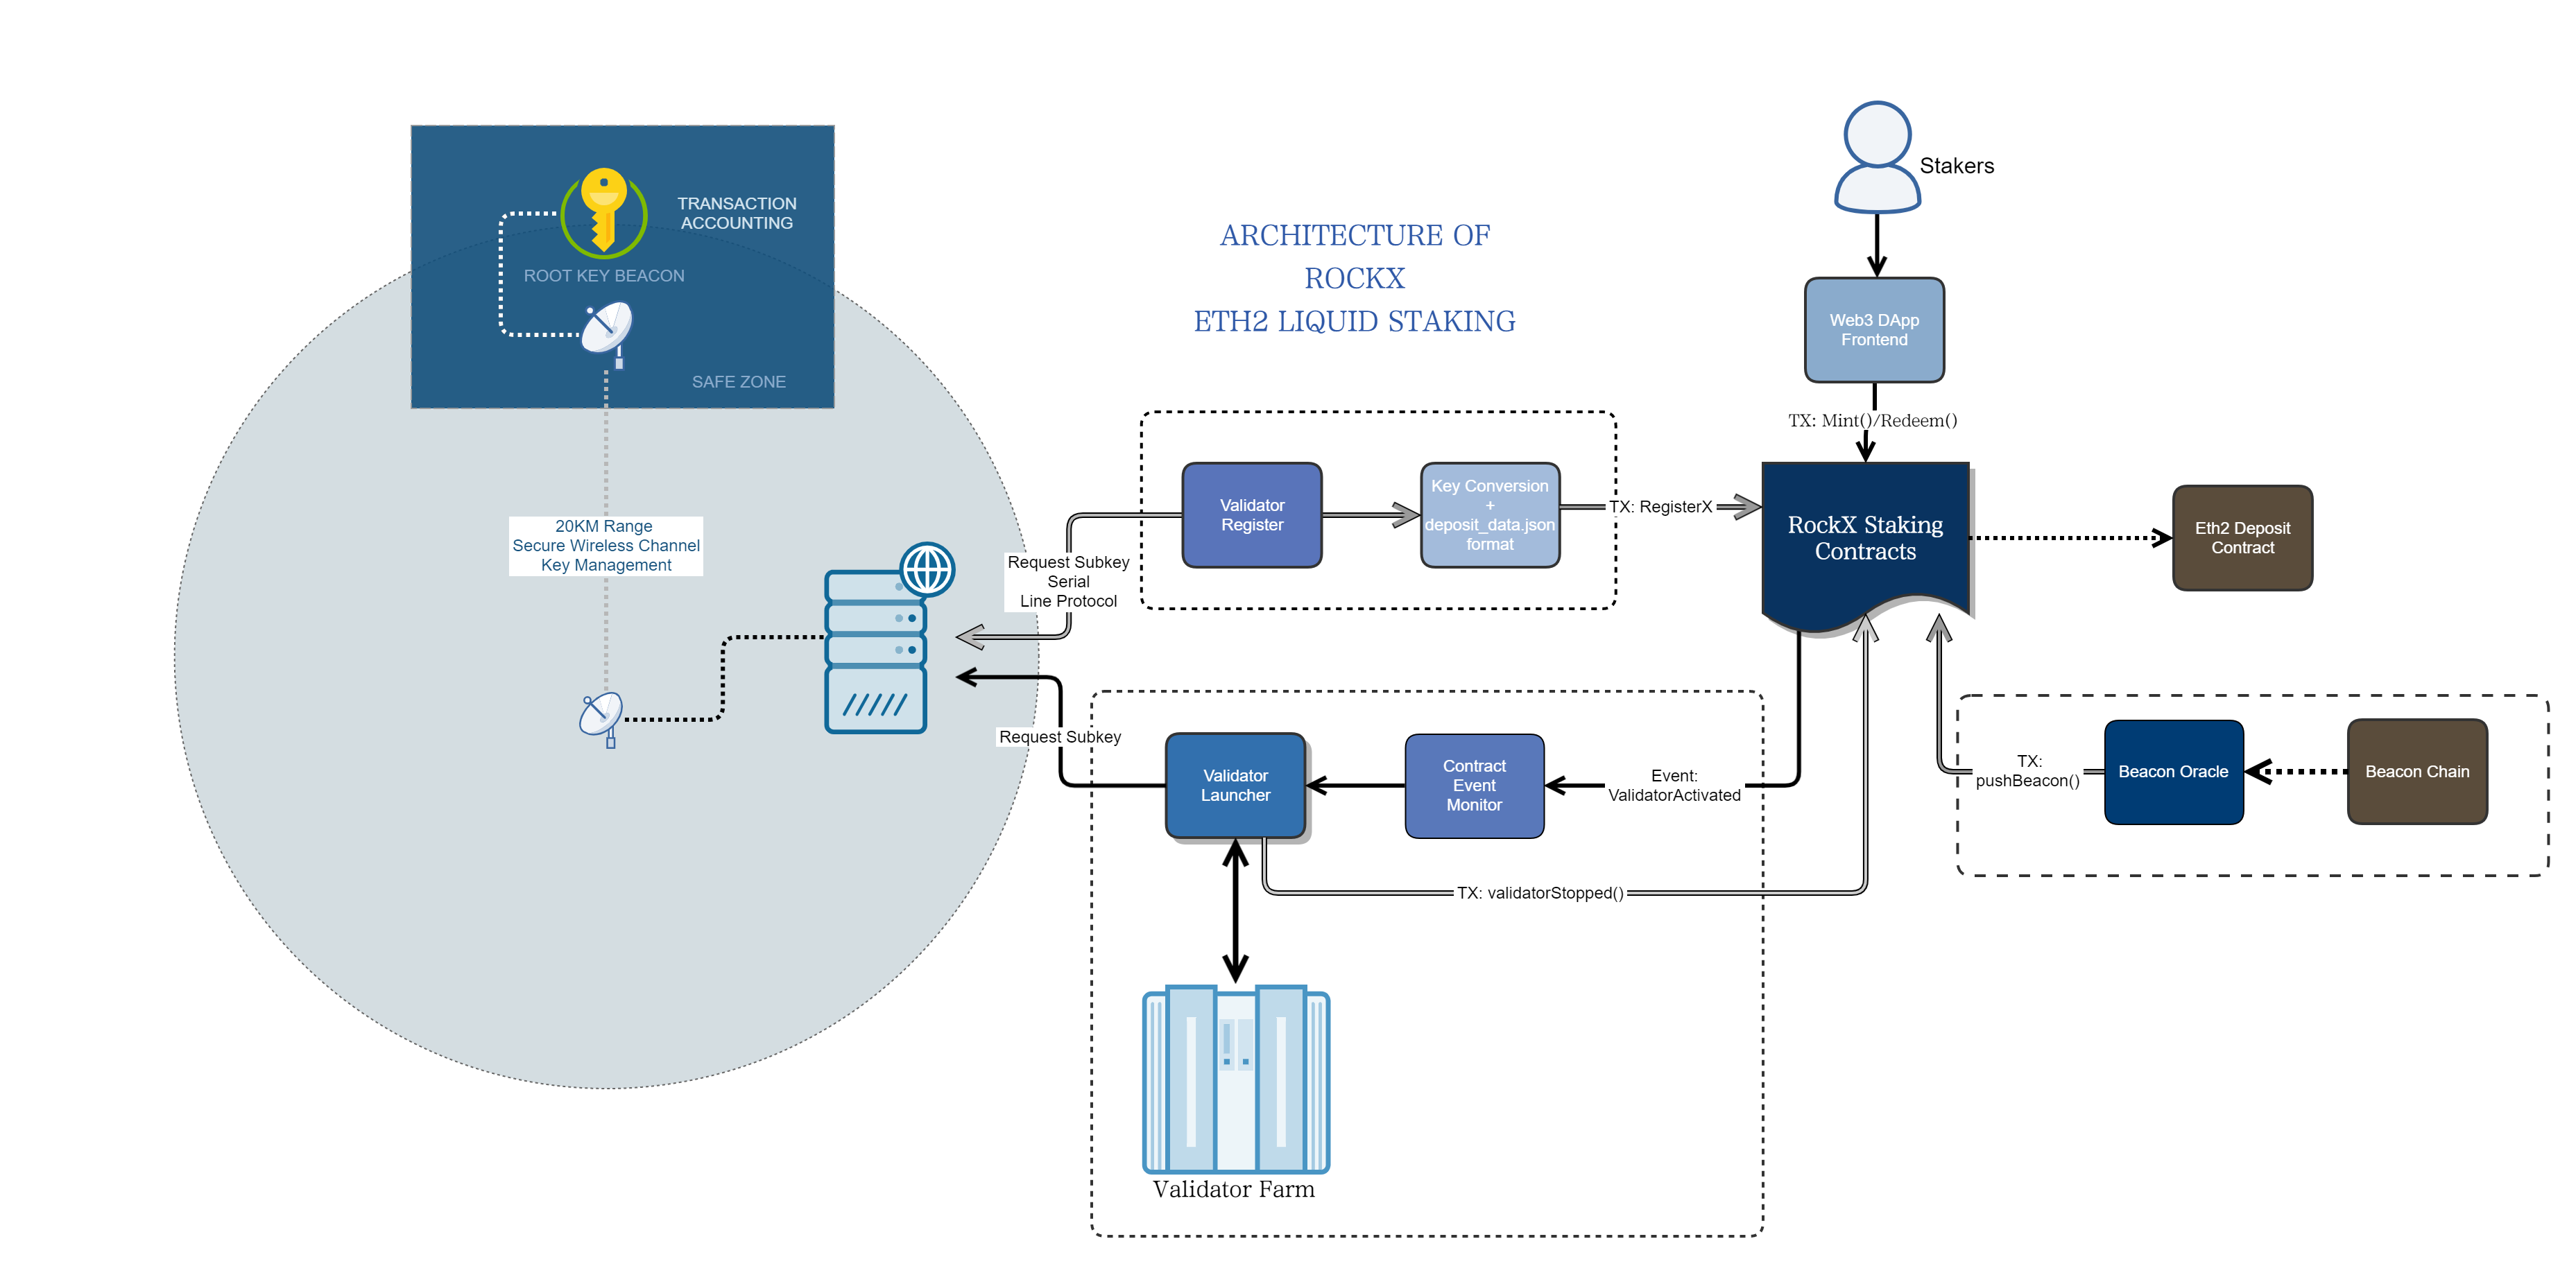
\includegraphics[scale=0.17, angle=270]{arch.png}
\end{figure}

\end{document}